\justifying \small 

\textcolor{cyan}{typedef} 
\textcolor{cyan}{unsigned} 
\textcolor{cyan}{char} 
\textcolor{white}{bit} 
\textcolor{magenta}{;} 
\textcolor{cyan}{struct} 
\textcolor{white}{Nodo} 
\textcolor{yellow}{*} 
\textcolor{white}{primero} 
\textcolor{yellow}{=} 
\textcolor{white}{NULL} 
\textcolor{magenta}{;} 
\textcolor{cyan}{struct} 
\textcolor{white}{Persona} 
\textcolor{magenta}{\{} 
\textcolor{cyan}{char} 
\textcolor{yellow}{*} 
\textcolor{white}{nombre} 
\textcolor{magenta}{;} 
\textcolor{cyan}{int} 
\textcolor{white}{edad} 
\textcolor{magenta}{;} 
\textcolor{white}{bit} 
\textcolor{white}{id} 
\textcolor{magenta}{;} 
\textcolor{magenta}{\}} 
\textcolor{magenta}{;} 
\textcolor{cyan}{struct} 
\textcolor{white}{Nodo} 
\textcolor{magenta}{\{} 
\textcolor{cyan}{struct} 
\textcolor{white}{Persona} 
\textcolor{white}{persona} 
\textcolor{magenta}{;} 
\textcolor{cyan}{struct} 
\textcolor{white}{Nodo} 
\textcolor{yellow}{*} 
\textcolor{white}{sig} 
\textcolor{magenta}{;} 
\textcolor{magenta}{\}} 
\textcolor{magenta}{;} 
\textcolor{cyan}{void} 
\textcolor{white}{agregarPersona} 
\textcolor{magenta}{(} 
\textcolor{cyan}{const} 
\textcolor{cyan}{char} 
\textcolor{yellow}{*} 
\textcolor{white}{nombre} 
\textcolor{magenta}{,} 
\textcolor{cyan}{int} 
\textcolor{white}{edad} 
\textcolor{magenta}{,} 
\textcolor{white}{bit} 
\textcolor{white}{id} 
\textcolor{magenta}{)} 
\textcolor{magenta}{\{} 
\textcolor{cyan}{struct} 
\textcolor{white}{Nodo} 
\textcolor{yellow}{*} 
\textcolor{white}{nuevo} 
\textcolor{yellow}{=} 
\textcolor{magenta}{(} 
\textcolor{cyan}{struct} 
\textcolor{white}{Nodo} 
\textcolor{yellow}{*} 
\textcolor{magenta}{)} 
\textcolor{white}{malloc} 
\textcolor{magenta}{(} 
\textcolor{cyan}{sizeof} 
\textcolor{magenta}{(} 
\textcolor{cyan}{struct} 
\textcolor{white}{Nodo} 
\textcolor{magenta}{)} 
\textcolor{magenta}{)} 
\textcolor{magenta}{;} 
\textcolor{white}{nuevo} 
\textcolor{yellow}{->} 
\textcolor{white}{sig} 
\textcolor{yellow}{=} 
\textcolor{white}{NULL} 
\textcolor{magenta}{;} 
\textcolor{white}{nuevo} 
\textcolor{yellow}{->} 
\textcolor{white}{persona} 
\textcolor{yellow}{.} 
\textcolor{white}{nombre} 
\textcolor{yellow}{=} 
\textcolor{magenta}{(} 
\textcolor{cyan}{char} 
\textcolor{yellow}{*} 
\textcolor{magenta}{)} 
\textcolor{white}{malloc} 
\textcolor{magenta}{(} 
\textcolor{green}{1} 
\textcolor{magenta}{)} 
\textcolor{magenta}{;} 
\textcolor{white}{strcpy} 
\textcolor{magenta}{(} 
\textcolor{white}{nuevo} 
\textcolor{yellow}{->} 
\textcolor{white}{persona} 
\textcolor{yellow}{.} 
\textcolor{white}{nombre} 
\textcolor{magenta}{,} 
\textcolor{white}{nombre} 
\textcolor{magenta}{)} 
\textcolor{magenta}{;} 
\textcolor{white}{nuevo} 
\textcolor{yellow}{->} 
\textcolor{white}{persona} 
\textcolor{yellow}{.} 
\textcolor{white}{edad} 
\textcolor{yellow}{=} 
\textcolor{white}{edad} 
\textcolor{magenta}{;} 
\textcolor{white}{nuevo} 
\textcolor{yellow}{->} 
\textcolor{white}{persona} 
\textcolor{yellow}{.} 
\textcolor{white}{id} 
\textcolor{yellow}{=} 
\textcolor{white}{id} 
\textcolor{magenta}{;} 
\textcolor{cyan}{if} 
\textcolor{magenta}{(} 
\textcolor{white}{primero} 
\textcolor{yellow}{==} 
\textcolor{white}{NULL} 
\textcolor{magenta}{)} 
\textcolor{magenta}{\{} 
\textcolor{white}{primero} 
\textcolor{yellow}{=} 
\textcolor{white}{nuevo} 
\textcolor{magenta}{;} 
\textcolor{magenta}{\}} 
\textcolor{cyan}{else} 
\textcolor{magenta}{\{} 
\textcolor{white}{nuevo} 
\textcolor{yellow}{->} 
\textcolor{white}{sig} 
\textcolor{yellow}{=} 
\textcolor{white}{primero} 
\textcolor{magenta}{;} 
\textcolor{white}{primero} 
\textcolor{yellow}{=} 
\textcolor{white}{nuevo} 
\textcolor{magenta}{;} 
\textcolor{magenta}{\}} 
\textcolor{magenta}{\}} 
\textcolor{cyan}{unsigned} 
\textcolor{cyan}{char} 
\textcolor{white}{aislarBit} 
\textcolor{magenta}{(} 
\textcolor{cyan}{int} 
\textcolor{white}{n} 
\textcolor{magenta}{,} 
\textcolor{cyan}{unsigned} 
\textcolor{cyan}{char} 
\textcolor{white}{ID} 
\textcolor{magenta}{)} 
\textcolor{magenta}{\{} 
\textcolor{cyan}{unsigned} 
\textcolor{cyan}{char} 
\textcolor{white}{bit} 
\textcolor{yellow}{=} 
\textcolor{white}{ID} 
\textcolor{magenta}{;} 
\textcolor{white}{bit} 
\textcolor{yellow}{=} 
\textcolor{white}{bit} 
\textcolor{yellow}{<<} 
\textcolor{magenta}{(} 
\textcolor{white}{n} 
\textcolor{green}{-1} 
\textcolor{magenta}{)} 
\textcolor{magenta}{;} 
\textcolor{white}{bit} 
\textcolor{yellow}{=} 
\textcolor{white}{bit} 
\textcolor{yellow}{>>} 
\textcolor{green}{7} 
\textcolor{magenta}{;} 
\textcolor{cyan}{return} 
\textcolor{white}{bit} 
\textcolor{magenta}{;} 
\textcolor{magenta}{\}} 
\textcolor{cyan}{void} 
\textcolor{white}{imprimir} 
\textcolor{magenta}{(} 
\textcolor{magenta}{)} 
\textcolor{magenta}{\{} 
\textcolor{white}{puts} 
\textcolor{magenta}{(} 
\textcolor{green}{"\textbackslash nLista de personas:\textbackslash n"} 
\textcolor{magenta}{)} 
\textcolor{magenta}{;} 
\textcolor{cyan}{struct} 
\textcolor{white}{Nodo} 
\textcolor{yellow}{*} 
\textcolor{white}{aux} 
\textcolor{yellow}{=} 
\textcolor{white}{primero} 
\textcolor{magenta}{;} 
\textcolor{cyan}{while} 
\textcolor{magenta}{(} 
\textcolor{white}{aux} 
\textcolor{yellow}{!=} 
\textcolor{white}{NULL} 
\textcolor{magenta}{)} 
\textcolor{magenta}{\{} 
\textcolor{white}{printf} 
\textcolor{magenta}{(} 
\textcolor{green}{"Nombre: \%s, Edad: \%i, ID: \%i, Bit2: \%d\textbackslash n"} 
\textcolor{magenta}{,} 
\textcolor{white}{aux} 
\textcolor{yellow}{->} 
\textcolor{white}{persona} 
\textcolor{yellow}{.} 
\textcolor{white}{nombre} 
\textcolor{magenta}{,} 
\textcolor{white}{aux} 
\textcolor{yellow}{->} 
\textcolor{white}{persona} 
\textcolor{yellow}{.} 
\textcolor{white}{edad} 
\textcolor{magenta}{,} 
\textcolor{white}{aux} 
\textcolor{yellow}{->} 
\textcolor{white}{persona} 
\textcolor{yellow}{.} 
\textcolor{white}{id} 
\textcolor{magenta}{,} 
\textcolor{white}{aislarBit} 
\textcolor{magenta}{(} 
\textcolor{green}{2} 
\textcolor{magenta}{,} 
\textcolor{white}{aux} 
\textcolor{yellow}{->} 
\textcolor{white}{persona} 
\textcolor{yellow}{.} 
\textcolor{white}{id} 
\textcolor{magenta}{)} 
\textcolor{magenta}{)} 
\textcolor{magenta}{;} 
\textcolor{white}{aux} 
\textcolor{yellow}{=} 
\textcolor{white}{aux} 
\textcolor{yellow}{->} 
\textcolor{white}{sig} 
\textcolor{magenta}{;} 
\textcolor{magenta}{\}} 
\textcolor{magenta}{\}} 
\textcolor{cyan}{int} 
\textcolor{white}{main} 
\textcolor{magenta}{(} 
\textcolor{magenta}{)} 
\textcolor{magenta}{\{} 
\textcolor{white}{agregarPersona} 
\textcolor{magenta}{(} 
\textcolor{green}{"Ronald"} 
\textcolor{magenta}{,} 
\textcolor{green}{21} 
\textcolor{magenta}{,} 
\textcolor{green}{12} 
\textcolor{magenta}{)} 
\textcolor{magenta}{;} 
\textcolor{white}{agregarPersona} 
\textcolor{magenta}{(} 
\textcolor{green}{"Rose"} 
\textcolor{magenta}{,} 
\textcolor{green}{18} 
\textcolor{magenta}{,} 
\textcolor{green}{13} 
\textcolor{magenta}{)} 
\textcolor{magenta}{;} 
\textcolor{white}{agregarPersona} 
\textcolor{magenta}{(} 
\textcolor{green}{"Ashly"} 
\textcolor{magenta}{,} 
\textcolor{green}{17} 
\textcolor{magenta}{,} 
\textcolor{green}{12} 
\textcolor{magenta}{)} 
\textcolor{magenta}{;} 
\textcolor{white}{agregarPersona} 
\textcolor{magenta}{(} 
\textcolor{green}{"Jack"} 
\textcolor{magenta}{,} 
\textcolor{green}{14} 
\textcolor{magenta}{,} 
\textcolor{green}{18} 
\textcolor{magenta}{)} 
\textcolor{magenta}{;} 
\textcolor{white}{agregarPersona} 
\textcolor{magenta}{(} 
\textcolor{green}{"Chester"} 
\textcolor{magenta}{,} 
\textcolor{green}{13} 
\textcolor{magenta}{,} 
\textcolor{green}{21} 
\textcolor{magenta}{)} 
\textcolor{magenta}{;} 
\textcolor{white}{agregarPersona} 
\textcolor{magenta}{(} 
\textcolor{green}{"Mike"} 
\textcolor{magenta}{,} 
\textcolor{green}{12} 
\textcolor{magenta}{,} 
\textcolor{green}{32} 
\textcolor{magenta}{)} 
\textcolor{magenta}{;} 
\textcolor{white}{agregarPersona} 
\textcolor{magenta}{(} 
\textcolor{green}{"Jen"} 
\textcolor{magenta}{,} 
\textcolor{green}{38} 
\textcolor{magenta}{,} 
\textcolor{green}{21} 
\textcolor{magenta}{)} 
\textcolor{magenta}{;} 
\textcolor{white}{imprimir} 
\textcolor{magenta}{(} 
\textcolor{magenta}{)} 
\textcolor{magenta}{;} 
\textcolor{cyan}{return} 
\textcolor{green}{0} 
\textcolor{magenta}{;} 
\textcolor{magenta}{\}} 




\begin{frame}{Histograma Tokens Usados} 
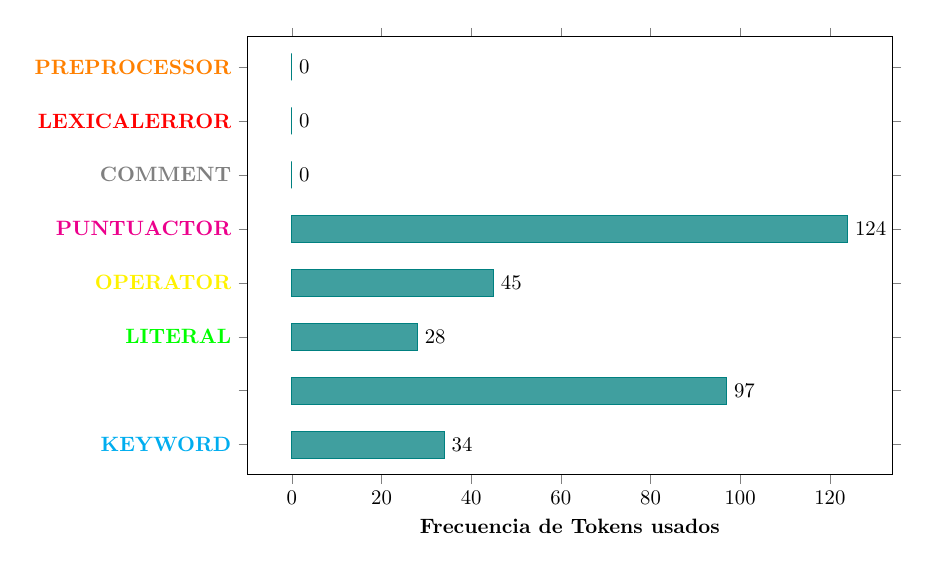
\begin{tikzpicture}[scale=0.75] % tamaño 
\begin{axis}[xbar,tick align=outside, 
    width=12.5cm,       % largo 
    height=9cm,       % altura 
    bar width={13pt},   % grosor linea 
    enlargelimits=0.08, % cercania a linea 
    nodes near coords, 
    nodes near coords align=horizontal, 
    point meta=x * 1, % The displayed number. 
    xlabel=\textbf{Frecuencia de Tokens usados}, 
    ytick={0,...,7}, 
    yticklabels={ 
        \textcolor{cyan}{\textbf{KEYWORD}},         % POSITION 0 
        \textcolor{white}{\textbf{IDENTIFIER}},     % POSITION 1 
        \textcolor{green}{\textbf{LITERAL}},        % POSITION 2 
        \textcolor{yellow}{\textbf{OPERATOR}},      % POSITION 3 
        \textcolor{magenta}{\textbf{PUNTUACTOR}},   % POSITION 4 
        \textcolor{gray}{\textbf{COMMENT}},         % POSITION 5 
        \textcolor{red}{\textbf{LEXICALERROR}},     % POSITION 6 
        \textcolor{orange}{\textbf{PREPROCESSOR}}   % POSITION 7 
    }] 
\addplot 
[draw=teal,fill=teal!75] 
coordinates {(34,0) (97,1) (28,2) (45,3) (124,4) (0,5) (0,6) (0,7)}; 
\end{axis}
\end{tikzpicture}
\end{frame}
